
%%%%%%%%%%%%%%%%%%%%%%% file typeinst.tex %%%%%%%%%%%%%%%%%%%%%%%%%
%
% This is the LaTeX source for the instructions to authors using
% the LaTeX document class 'llncs.cls' for contributions to
% the Lecture Notes in Computer Sciences series.
% http://www.springer.com/lncs       Springer Heidelberg 2006/05/04
%
% It may be used as a template for your own input - copy it
% to a new file with a new name and use it as the basis
% for your article.
%
% NB: the document class 'llncs' has its own and detailed documentation, see
% ftp://ftp.springer.de/data/pubftp/pub/tex/latex/llncs/latex2e/llncsdoc.pdf
%
%%%%%%%%%%%%%%%%%%%%%%%%%%%%%%%%%%%%%%%%%%%%%%%%%%%%%%%%%%%%%%%%%%%


\documentclass[runningheads,a4paper,spanish]{llncs}
\usepackage{listings}
\usepackage[utf8]{inputenc}
\usepackage{amssymb}
\usepackage{url}
\usepackage{graphicx}
\usepackage{float}
\DeclareGraphicsExtensions{.png,.jpg}
\usepackage[spanish]{babel}
\usepackage{selinput}
\usepackage{appendix}
\renewcommand{\appendixname}{Anexos}
\renewcommand{\appendixtocname}{Anexos}
\renewcommand{\appendixpagename}{Anexos}
\selectlanguage{spanish}
\setcounter{tocdepth}{3}


\urldef{\mailsa}\path|pnavarro@fi.uba.ar,|
\urldef{\mailsb}\path|magual89@gmail.com,|   
\newcommand{\keywords}[1]{\par\addvspace\baselineskip
\noindent\keywordname\enspace\ignorespaces#1}

\begin{document}

\mainmatter  % start of an individual contribution

% first the title is needed
\title{Nutri Dietas:\\
Trabajo Profesional de Ingenieria\\
en Informatica. Universidad\\
de Buenos Aires}

% a short form should be given in case it is too long for the running head
\titlerunning{Nutri Dietas}

% the name(s) of the author(s) follow(s) next
%
% NB: Chinese authors should write their first names(s) in front of
% their surnames. This ensures that the names appear correctly in
% the running heads and the author index.
%
\author{Navarro Patricio \and Alvarez Matias Agustin}
%
\authorrunning{Nutri Salud: Trabajo Profesional}
% (feature abused for this document to repeat the title also on left hand pages)

% the affiliations are given next; don't give your e-mail address
% unless you accept that it will be published
\institute{Universidad de Buenos Aires,\\
Facultad de Ingenieria\\
\mailsa\\
\mailsb\\
\url{http://www.fi.uba.ar}}

%
% NB: a more complex sample for affiliations and the mapping to the
% corresponding authors can be found in the file "llncs.dem"
% (search for the string "\mainmatter" where a contribution starts).
% "llncs.dem" accompanies the document class "llncs.cls".
%

\toctitle{Nutri Salud}
\tocauthor{Trabajo Profesional}
\maketitle


\begin{abstract}
Trabajo Profesional de la carrera Ingeniería en Informática de la Universidad de Buenos Aires. Se 
desarrollo un sistema de gestión de pacientes para un profesional de la nutrición, orientado a administrar tanto dietas y pacientes como los turnos del profesional. El sistema se realizo enteramente para funcionar sobre una plataforma Web.
\keywords{Nutrición, Gestion, Ruby on Rails, Salud}
\end{abstract}


\section{Introducion}

La Universidad de Buenos Aires (UBA) se creó en 1821, a cinco años de la declaración
de la independencia. En 1865 se crea el Departamento de Ciencias Exactas,
que se dedica a \textit{“… la enseñanza de las matemáticas puras y aplicadas, y de la historia
natural"}. En 1866 hay trece inscriptos y el primer graduado es Luis Augusto Huergo,
que recibe su diploma de \textit{“Ingeniero de la Escuela de esta Universidad en la
Facultad de Ciencias Exactas"}. El Ing. Huergo es así el primer ingeniero graduado
en el país.

En el año 1952 se separaron las carreras dando lugar a la creación de la Facultad
de Ingeniería, que actualmente desarrolla sus actividades en tres sedes en la Ciudad
de Buenos Aires.

La Facultad de Ingeniería tiene como objetivo formar profesionales de la más alta
calidad y compromiso cívico y profesional para contribuir de manera destacada al
desarrollo sustentable de las economías regionales, el fortalecimiento de la soberanía
nacional y al posicionamiento de la Argentina en el ámbito internacional.

La profesión de Ingeniero implica fundamentalmente la capacidad de resolver
problemas de naturaleza tecnológica ligados a la concepción, diseño, realización y
fabricación de productos, sistemas o servicios, así como contribuir a la investigación
y desarrollo de nuevas tecnologías. La formación profesional requerida debe tener en
cuenta además los continuos cambios de la ciencia y la tecnología así como los
cambios en los esquemas económicos, productivos y sociales en nuestro país y el
resto del mundo.\cite{carrera}

Dentro del marco de esta institución hemos realizado nuestro trabajo profesional de la carrera Ingeniería Informática, cumpliendo con todos los requisitos impuestos por la universidad, así como realizando un trabajo a un particular, el cual cumple con los mas altos estándares profesionales del momento. Este trabajo ha sido tutelado y validado por el Ingeniero Arturo Servetto, profesor adjunto con dedicación exclusiva, miembro de la Comisión Curricular Permanente de la carrera de Ingeniería en Informática y director del Laboratorio de Sistemas Operativos y Bases de Datos, en la facultad de Ingeniería de la Universidad de Buenos Aires.


\section{Objetivo}
El objetivo de este proyecto es desarrollar un sistema que posibilite la gestión de pacientes y dietas de la Lic. Mercedes Gabín, permitiendo también realizar el seguimiento de los pacientes de forma remota y visualizar estadísticas sobre el progreso de los mismos.  Es también parte de nuestro objetivo, en el desarrollo personal como futuros profesionales en el campo de la Ingeniería Informática, el conocer y manejar distintas herramientas que nos permitan cumplir con el perfil del graduado requerido por la Universidad de Buenos Aires (UBA).
\cite{computacion}

\begin{quotation}
	\textit{PERFIL DEL GRADUADO: El Ingeniero en Informática se caracteriza por poseer una sólida formación en el área
	de la informática en general y en una de sus ramas de especialización, a su elección,
	en particular. Está capacitado, debido a los fundamentos que adquiere en la carrera,
	la extensa práctica en la que se involucra, y el aprendizaje de tecnología de última
	generación, a comprender los problemas del mundo real para diseñar y aplicar la
	solución informática que mejor se ajuste a cada problema concreto, integrándola al
	resto de los procesos. Podrá entonces encarar problemas de alta complejidad y de
	naturaleza diversa con conocimiento y capacidad analítica para construir su solución
	computacional de forma científica con el uso de herramientas avanzadas, adecuadas
	al estado del arte en computación, aplicando sus conocimientos de forma independiente,
	crítica e innovadora. Su formación le permite adaptarse a la dinámica organizacional,
	aplicando su formación en gestión, su entrenamiento para el trabajo en
	grupo y sus habilidades de comunicación y expresión.}\cite{carrera}
\end{quotation}


\section{Descripción del problema}
Nos encontramos con un profesional de la salud, Licenciada en Nutrición Mercedes Gabin, la cual nos solicito un software capaz de facilitar su trabajo administrativo a la hora de trabajar con los distintos pacientes. El mismo debía encargarse de la administración de dietas y pacientes, como también de organizar y canalizar toda la interacción entre estos y el profesional. 

Se produjo una reunión con el cliente interesado en adquirir nuestros servicios, de la cual se desprendió una idea general del sistema requerido por el mismo, lo suficientemente detallada como para poder realizar algunos requerimientos funcionales y mockup del sistema. Una vez validados estos, se detallaron los casos de uso y se continuo a la solución del problema.

\subsection{Casos de uso}
El proceso de inserción del actor sistema pretende orientar al ingeniero de software a la captura de los requisitos de software utilizando los modelos de negocio. La estrategia consiste en determinar con el tipo de interacción que tiene cada uno de los actores que componen los modelos de negocios con el sistema de software.\cite{estrada}
\subsubsection{Administrador del sistema}
\begin{center}
	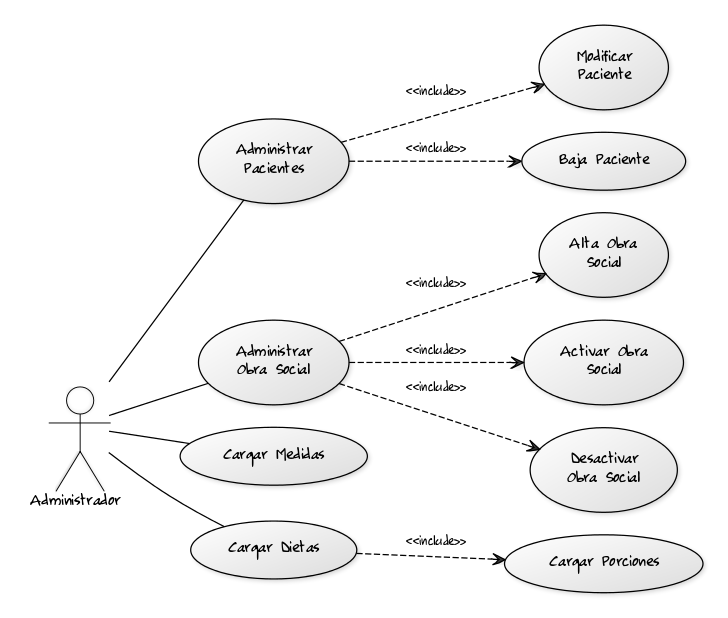
\includegraphics[scale=0.50]{Administrador}
\end{center}

\subsubsection{Paciente}
\begin{center}
	\includegraphics[scale=0.50]{Paciente}
\end{center}
\subsection{Requerimientos Funcionales}
\subsubsection{Proceso de gestión de pacientes}
El software debe permitir al administrador el alta, baja y modificación de los pacientes, así como conocer el estado de los mismos en cualquier momento (peso, medidas, objetivos, etc) a través de la web.
\subsubsection{Proceso de cálculo y visualización de índices por paciente}
El software debe proveer de forma automática el cálculo de distintos índices por paciente, en base a los datos aportados por el mismo o cargados manualmente por el administrador. 
\subsubsection{Proceso de gestión de obras sociales}
 El software debe permitir, al administrador, la gestión de las distintas obras sociales que admite, sin dejar en un estado invalido a aquellos pacientes que posean una obra social que ya no tiene convenio con el profesional.
\subsubsection{Proceso de gestión de dietas}
 El software debe permitir, al administrador, la posibilidad de cargar, modificar, eliminar y asignar dietas y objetivos a los distintos pacientes.
\subsubsection{Proceso de registración de pacientes}
El software debe permitir, al paciente, la posibilidad de registrarse al sistema de la licenciada, cargando sus datos personales. Este proceso da de alta el usuario en el sistema, así como le brinda la posibilidad de pedir un turno en un sistema previamente existente.
\subsubsection{Proceso de login de usuarios}
 El software debe permitir, al paciente, la posibilidad de ingresar a la plataforma para realizar los distintos procesos.
\subsubsection{Proceso de carga de datos semanales}
 El software debe permitir, al paciente, la posibilidad de ingresar su peso, distintas medidas corporales y objetivos semanalmente.
\subsubsection{Proceso de visualización de dieta}
 El software debe permitir, al paciente, la posibilidad de visualizar la dieta cargada por el administrador para dicha semana.
\subsubsection{Proceso de visualización de estadísticas}
 El software debe permitir, al paciente, la posibilidad de visualizar distintas estadísticas basadas en su historial.

\subsection{Sistema Previo}

El profesional contaba con un sistema preexistente para la administración de pacientes. Este se encontraba basado en una pagina web publica, en la cual los pacientes eran alentados a registrarse ya que esta era la única forma de obtener un turno con la licenciada. Una vez registrados, se generaba automáticamente un archivo de Excel con los datos provistos por el paciente el cual era utilizado a modo de “ficha personal" por el profesional. En dicha registracion, el usuario, debía proveer una clave personal, la cual en conjunto con su dirección de e-mail eran utilizados como credenciales en un sistema de administración de turnos online.

\section{Solución}

En vista de los requerimientos presentados por el cliente y de la estructura que este ya poseía se opto por implementar un sistema de gestión web atravez de Internet. Donde los pacientes pueden acceder 7x24 para consultar su “estado", el cual consiste en dietas , cantidades permitidas y gráficos de progreso. 

\subsection{Arquitectura}

En vista de la estructura previa existente, se tomo la desicion por reutilizar parte de esta estructura. El sistema de registro así como la generación del archivo Excel, serian reemplazados por completo, mientras que el sistema de turnos seria reutilizado en medida de lo posible.

El sistema web se realizo enteramente en Ruby on Rails, debido a las facilidades otorgadas por este framework de desarrollo, y a que se encuentra dentro del \textit{“estado del arte"} en desarrollo de este tipo de aplicaciones.

El framework Ruby on Rails está basado en el patŕon de arquitectura MVC, que consiste en separar las distintas responsabilidades del sistema entre clases de: Modelo, Vista y Controlador.
 
Otra característica importante es que Rails cumple con el principio de “convención por sobre configuración", esto quiere decir que si se mantienen ciertas reglas en cuanto a nombre de las clases y archivos que componen el sistema, queda minimizada en gran medida las configuraciones que uno debe realizar.

\subsubsection{Modelo}

Las entidades que forman parte del modelo, son las que representan una entidad de negocio, en ellas se especifican las restricciones que cada una de ellas presenta. Por ejemplo: valores prohibidos, rango de valores permitidos, unicidad.

Cada una de estas clases que representa a una entidad de negocio, que por lo general, tiene su correspondiente tabla en la base de datos.  Para realizar las consultas sobre las tablas asociadas a cada una de las clases del modelo, se utilizó la librería ActiveRecord, la cual cuenta con una gran cantidad de funciones y evita tener que realizar consultas SQL planas en la mayoría de los casos.

Los nombres de archivo que representan una clase del modelo, está formado por la entidad del negocio en singular, por ejemplo: "`diet.rb"', "`plan.rb"', "`user.rb"'.

\subsubsection{Vista}

Las clases que forman parte de la Vista, tienen como responsabilidad recibir los datos de negocio provenientes del controlador y proveer un formato adecuado para presentarlo.

Rails brinda facilidad para visualizar la información fácilmente en distintos formatos, ya sea JSON, XML o HTML.  Utilizando éste último en nuestro caso.

Para el diseño y la validación de ciertos campos desde la vista, se utilizaron librerías como Bootstrap, y tecnologías como Javascript.

Cabe destacar que se optó por un diseño diferente para la aplicación, dependiendo del rol del usuario autenticado en la misma,  teniendo así dos perfiles de aplicación: el de “Usuario Administrador” y el de “Usuario particular o Paciente".

Los nombres de archivo que representan una clase perteneciente a la vista, se colocan en una carpeta con el nombre de la entidad del modelo en plural: “diets", “plans", “users", y el nombre de archivo representa la acción del controlador de la cual recibe la información a ser presentada, por ejemplo: "`show.html.rb"', "`edit.html.rb"'.

\subsubsection{Controlador}

Cada entidad del negocio tiene un controlador asignado, el controlador es el encargado de decidir qué acción realizar en base a las peticiones HTTP que recibe el servidor.  Se encarga de obtener información de la base de datos, en caso de que sea necesario, y de enviar los datos a la vista cuando esto es necesario.

El controlador, nos permite, crear, modificar, modificar y listar las diferentes entidades que forman parte de nuestra aplicación.

En base a la URL, los parametros recibidos en el body de la petición HTTP y el method, se determina que acción del controlador debe actuar.

Las clases que forman parte del controlador, poseen la siguiente nomenclatura: nombre de la entidad en plural seguido de un guión bajo “\_" controller, por ejemplo: "`diets\_controller.rb"', "`plans\_controller.rb"', "`users\_controller.rb"'.


\subsection{Migracion de datos}
El nuevo sistema requería una migración de datos desde la antigua plataforma. Para realizar esto se utilizo un script en Python encargado de generar un archivo de texto por cada uno de los registros que el profesional poseía sobre cada paciente. Esto se combino con un script en bash encargado de separar los archivos bien parseados y unirlos en un único fichero para luego ser cargado en la base de datos.

\begin{verbatim}

\end{verbatim}

\subsection{Requerimientos no Funcionales}
En función de la solución realizada se determinaron los requisitos necesarios para la utilización del sistema por nosotros creado.
\subsubsection{Hardware}
Al ser una aplicación de índole web, los recursos a nivel hardware no son de gran escala. A continuación se detalla los requisitos mínimos:
\begin{itemize}
	\item \textit{Acceso a Internet}
	\item \textit{Procesador Intel Core 2 Duo}
	\item \textit{Memoria RAM 3 GB}
	\item \textit{Disco Rígido 220 GB}
\end{itemize}
\subsubsection{Software}
El sistema se desarrollada con independencia de plataforma por su condición de aplicación Web, es decir, podrá usarse en Windows, Linux, Mac los cuales soportan navegadores web:
	\begin{itemize}
		\item \textit{Google Chrome 19}
		\item \textit{Microsoft Internet Explorer 8}
		\item \textit{Firefox 12}
		\item \textit{Safari}
	\end{itemize}
\begin{flushleft}
	Por otro lado se usarán los siguientes lenguajes y Base de Datos: 
\end{flushleft}
	\begin{itemize}
		\item \textit{Ruby on Rails  V 4.1.8} 
		\item \textit{PostgreSQL}
		\item \textit{MySQL}
		\item \textit{Javascript }
		\item \textit{CSS}
		\item \textit{HTML}
		\item \textit{jQuery 1.8.1}
	\end{itemize}
\subsection{Herramientas de Desarrollo}
\subsubsection{Hardware}
[Detalle del equipamiento que se utilizará para desarrollar la aplicación]\\
El proyecto se realizara en una PC/Notebook con las siguientes especificaciones: 
	\begin{itemize}
		\item Procesador: \textit{Intel Core i.7}
		\item Disco Duro: \textit{1 TB}
		\item Memoria Ram: \textit{8gb}
	\end{itemize}
\subsubsection{Software}
Para el desarrollo del proyecto se usará el siguiente software:
	\begin{itemize}
		\item Entorno de desarrollo: \textit{Sublime 3}
		\item Sistema de control de versiones:\textit{ SVN, GIT}
		\item Framework: \textit{Ruby on Rails V 4.1.8 – Ruby}
		\item Lenguaje de programación Web:\textit{ HTML – CSS - Javascript - Ruby - JQuery}
		\item Sistema operativo: \textit{Linux}
		\item Motor de base de datos: \textit{PostgreSQL, MySql}
		\item Herramientas para la documentación del proyecto:  \textit{MS Word, Google Drive, \LaTeX{}}
		\item	Herramientas para desarrollo de diagramas: \textit{Draw.io}
		\item Herramientas para la gestión del proyecto: \textit{Trello}
	\end{itemize}
	
\section{Implementacion}
\subsection{Registración (Usuario)}
En esta sección el usuario deberá ingresar toda la información necesaria para que la Licenciada pueda realizar un correcto diagnóstico,  y así proveerle al paciente la dieta que más se adecúe a su situación actual. El usuario brinadará información acerca de sus hábitos o costumbres alimenticias, peso habitual, actual y deseado. Así como también la frecuencia y tipos de actividades físicas que realiza.\\
Por últimó son necesarios los datos personales del paciente, junto con una dirección de email, donde le llegará la confirmación de la registración a la plataforma y una contraseña para poder ingresar a la misma.

\subsection{Login (Usuario)}
Desde el portal de login, el usuario deberá ingresar el email que indicó en el proceso de registración y la contraseña correspondiente.  Cabe destacar que el usuario no podra loguearse en la plataforma sin previamente haber confirmado su cuenta vía email.
\begin{center}
	
\includegraphics[scale=0.3]{login.png}
\end{center}
\subsection{Dieta (Usuario)}
Desde aquí el usuario podrá visualizar las cantidades o porciones de cada uno de los tipos de alimentos especificados en las dietas, los cuales podrá consumir, en cada una de las distintas comidas: desayuno, almuerzo, merienda, cena, colación.
\begin{center}
	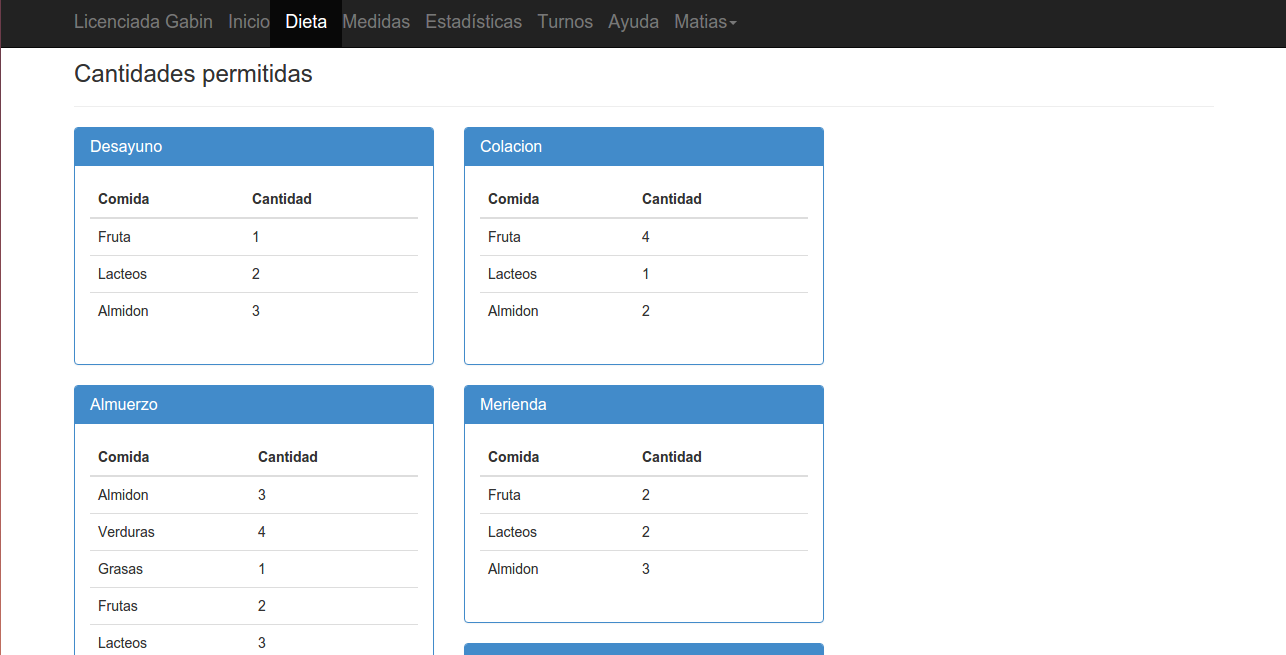
\includegraphics[scale=0.3]{dietas_cantidades.png}
\end{center}
\subsection{Medidas (Usuario)}
Desde la sección de Medidas el usuario, previa consulta al profesional, quedara habilitado para cargar sus medidas en casa. Datos que servirán para distintos cálculos y gráficos que efectuara la plataforma.
\begin{center}
	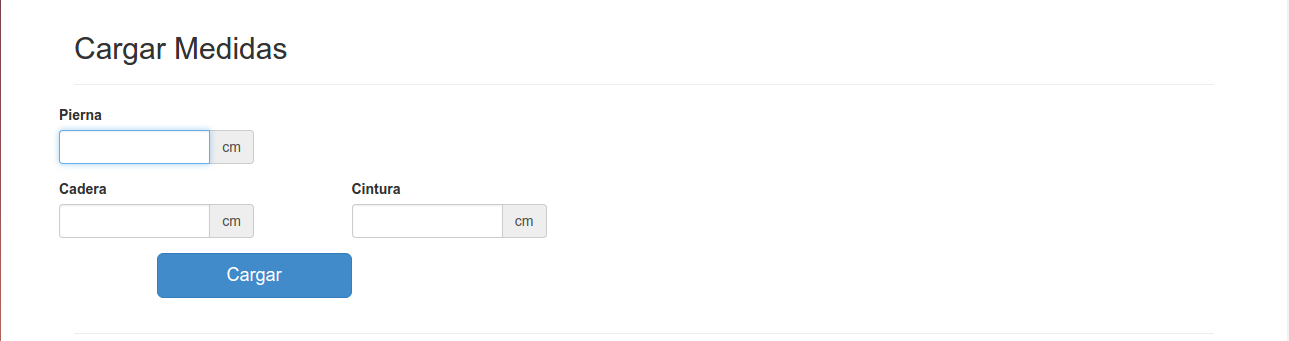
\includegraphics[scale=0.3]{carga_medidas_usuario.png}
\end{center}
\subsection{Estadísticas (Usuario)}
En esta sección el usuario puede observar cuales fueron sus ultimas medidas cargadas asi como el Riesgo de padecer enfermedades crónicas, indice de masa corporal y kg de grasa bruta.
\begin{center}
	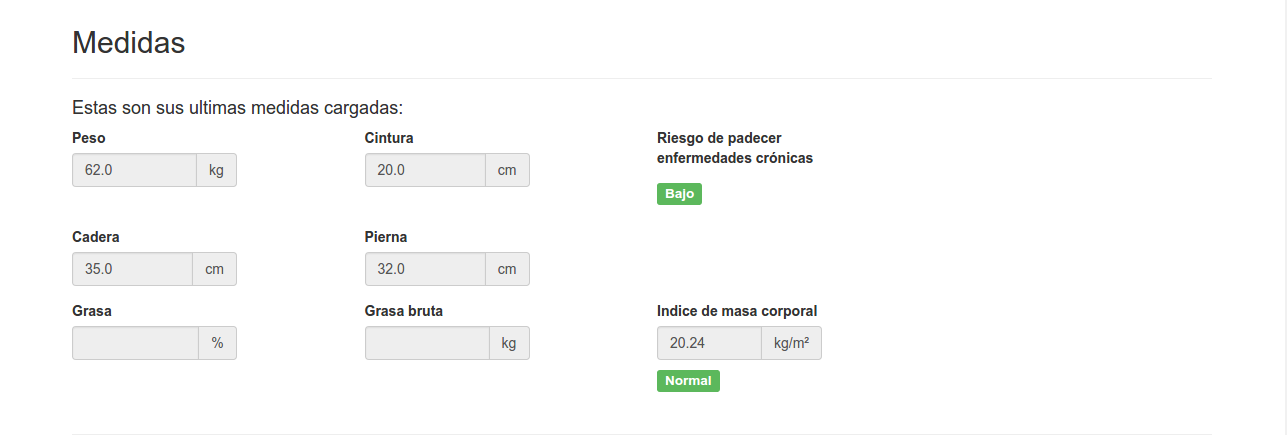
\includegraphics[scale=0.3]{ultimas_medidas.png}
\end{center}
Dentro de esta sección se encuentran los gráficos de progreso del usuario, entre ellos: Peso en función de tiempo; Grasa en función del tiempo; Cintura en función del tiempo; Etc.
\begin{center}
	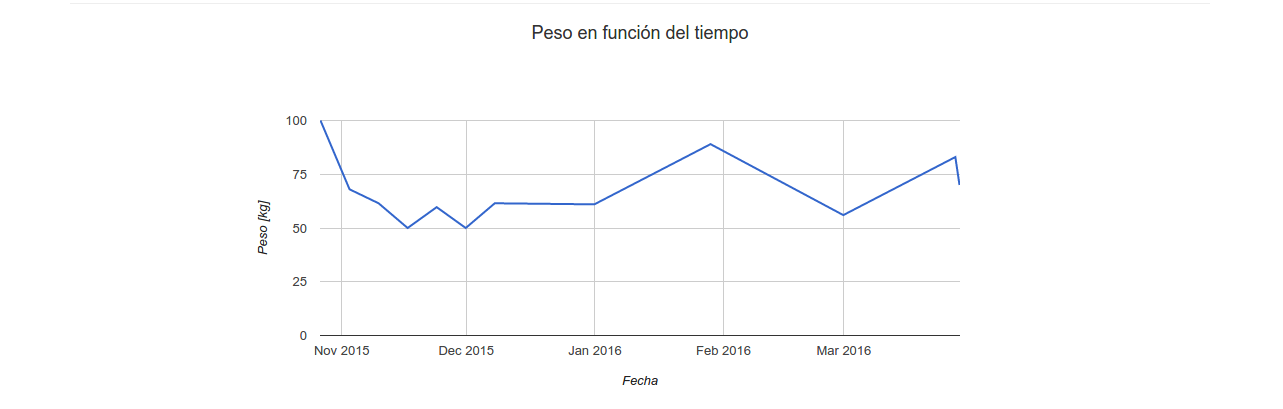
\includegraphics[scale=0.3]{grafico1.png}
\end{center}
\begin{center}
	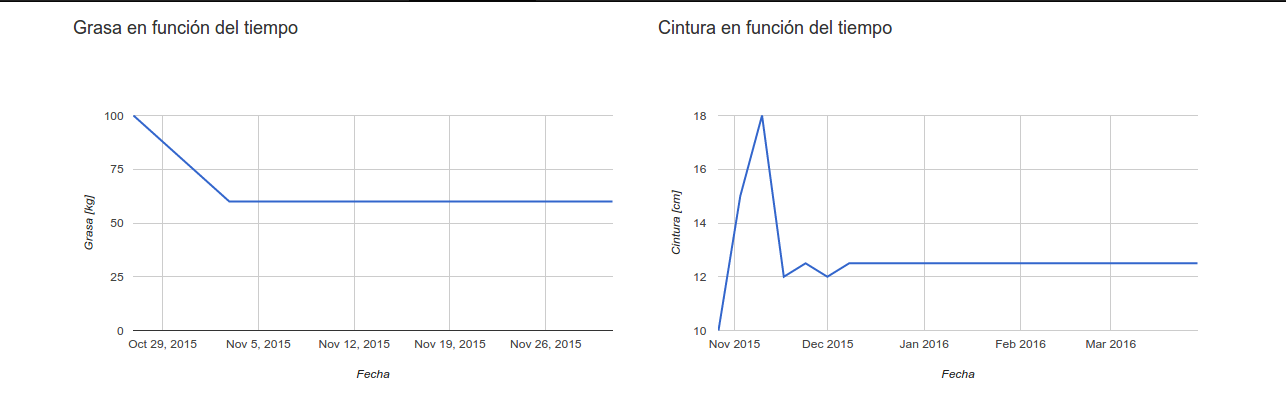
\includegraphics[scale=0.3]{grafico2.png}
\end{center}
\begin{center}
	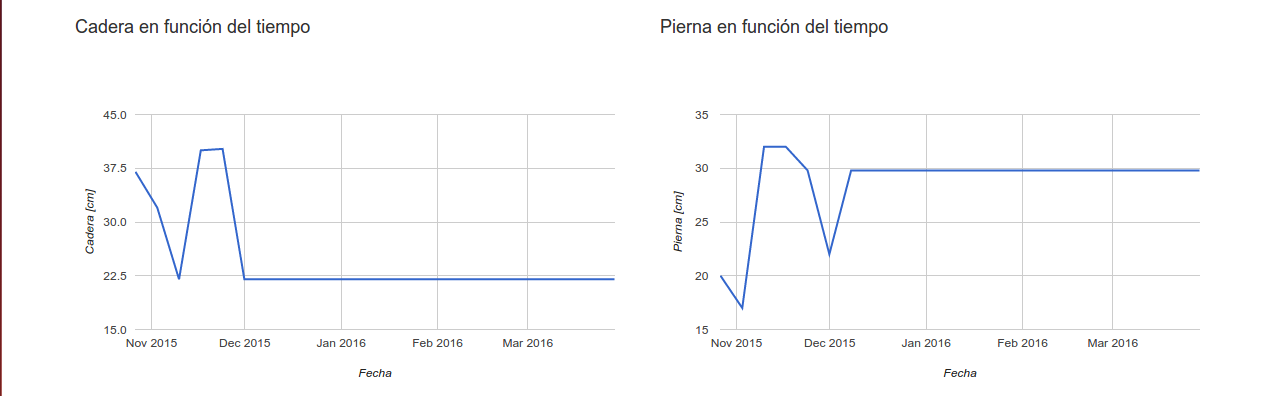
\includegraphics[scale=0.3]{grafico3.png}
\end{center}
\subsection{Ayuda (Usuario)}
En la sección de Ayuda se muestra un simple tutorial, explicando el funcionamiento de la plataforma, y en detalle cada una de sus secciones.
\begin{center}
	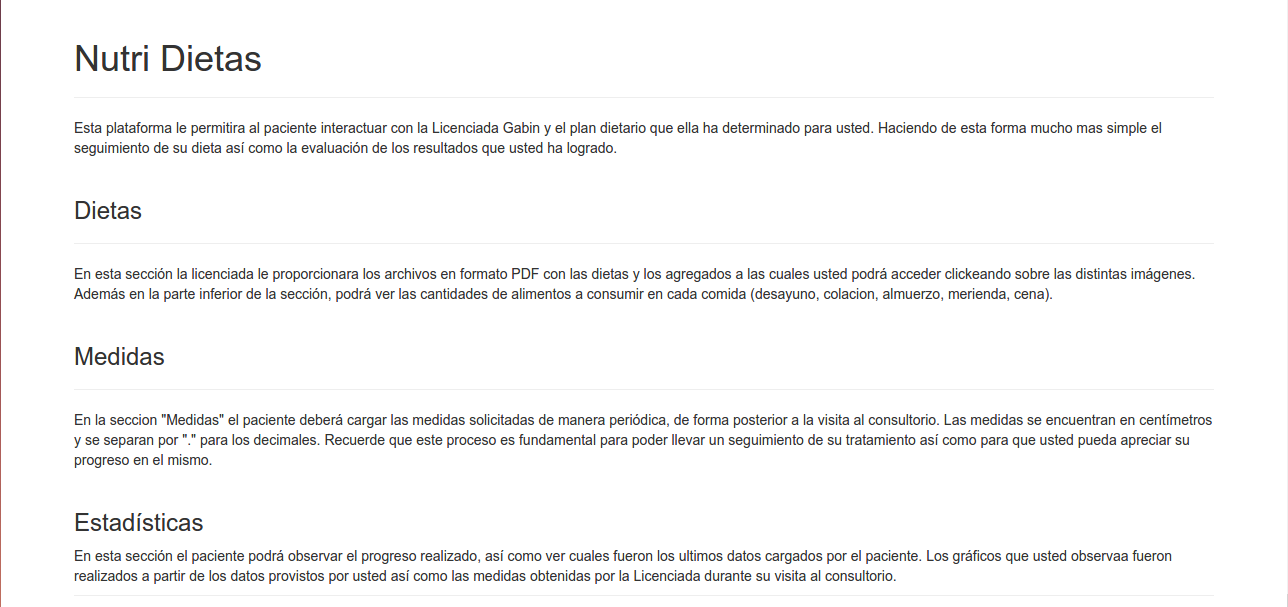
\includegraphics[scale=0.3]{help.png}
\end{center}

\subsection{Login (Administrador)}
Desde el portal de login, el administrador deberá ingresar el email y la contraseña correspondiente, este portal es distinto del portal de login de usuarios.  
\begin{center}
	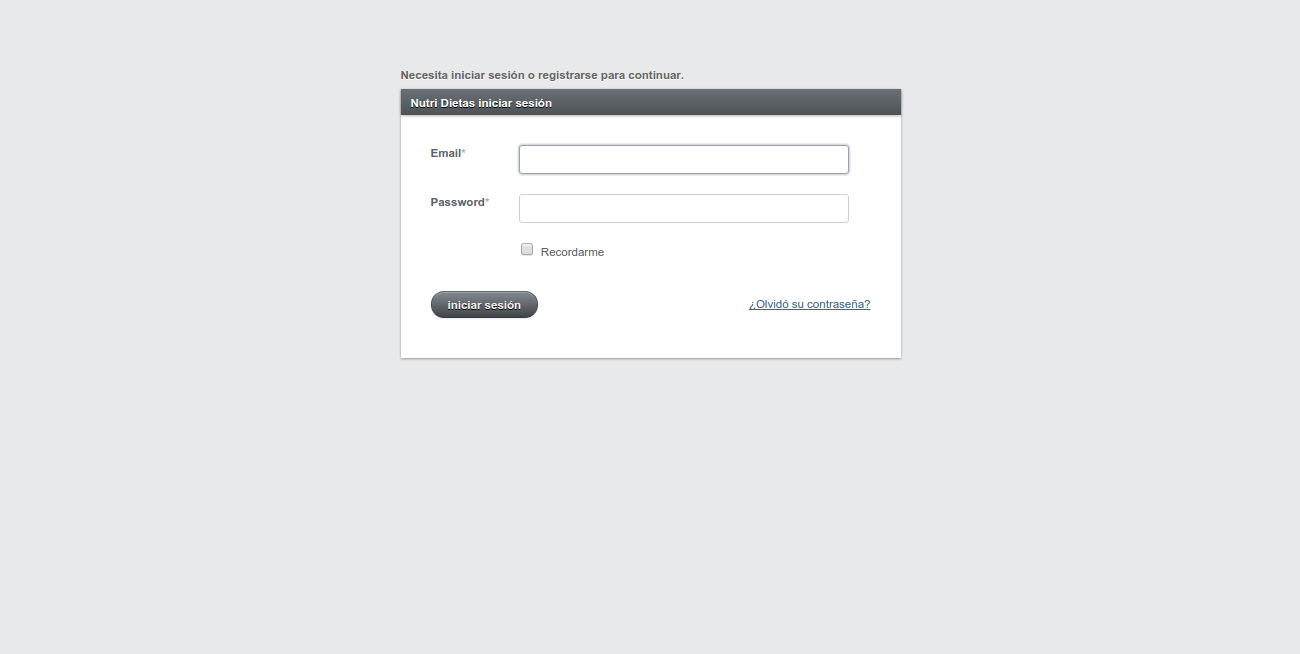
\includegraphics[scale=0.3]{admin_login.png}
\end{center}

\subsection{Usuarios administrador (Administrador)}
El administrador de la plataforma, puede a su vez agregar distintos usuarios administrador, para que cumplan un rol similar a este. En este caso el profesional, crea distintos usuarios para sus secretarias.
\begin{center}
	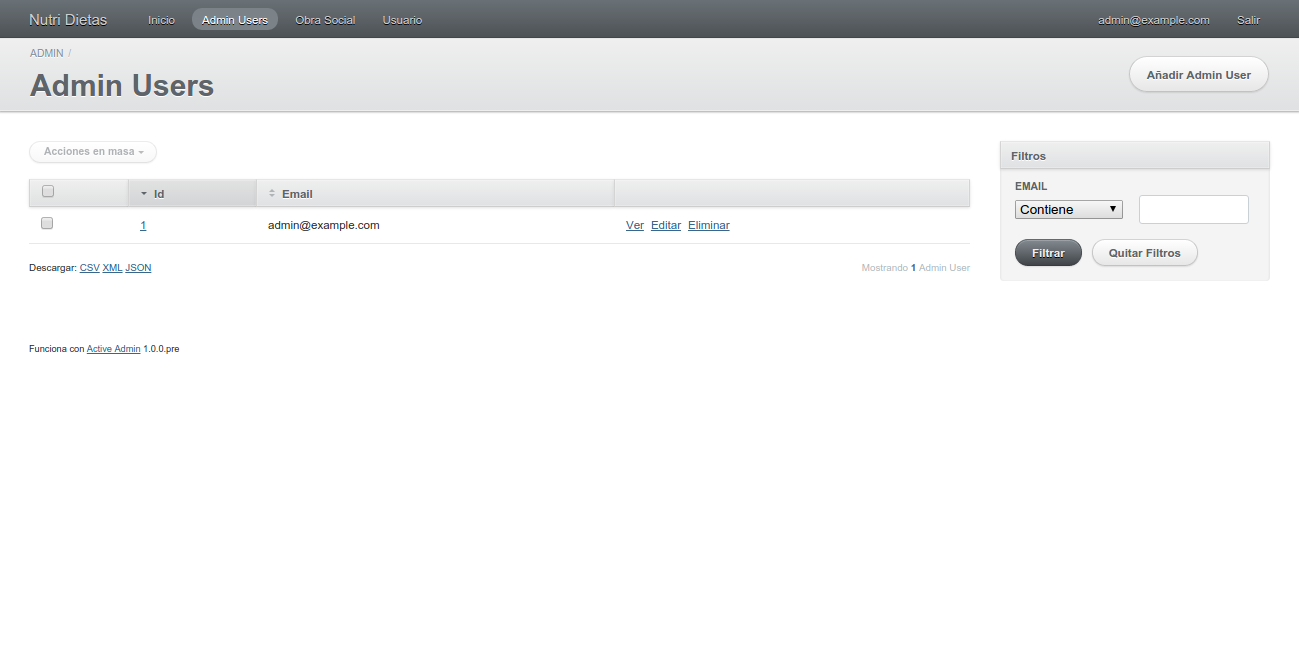
\includegraphics[scale=0.3]{admin_users.png}
\end{center}

\subsection{Dieta (Administrador)}
\begin{center}
	
\end{center}

\subsection{Cargar medidas (Aministrador)}
\begin{center}
	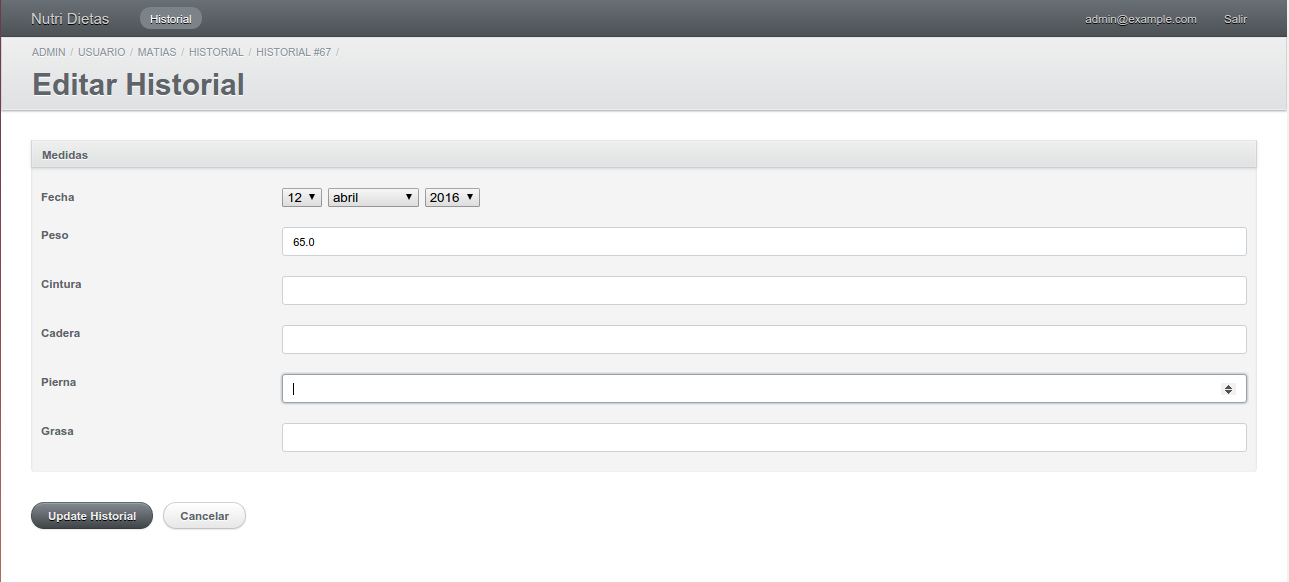
\includegraphics[scale=0.3]{cargar_medida.png}
\end{center}

\subsection{Paciente (Administrador)}
\begin{center}
	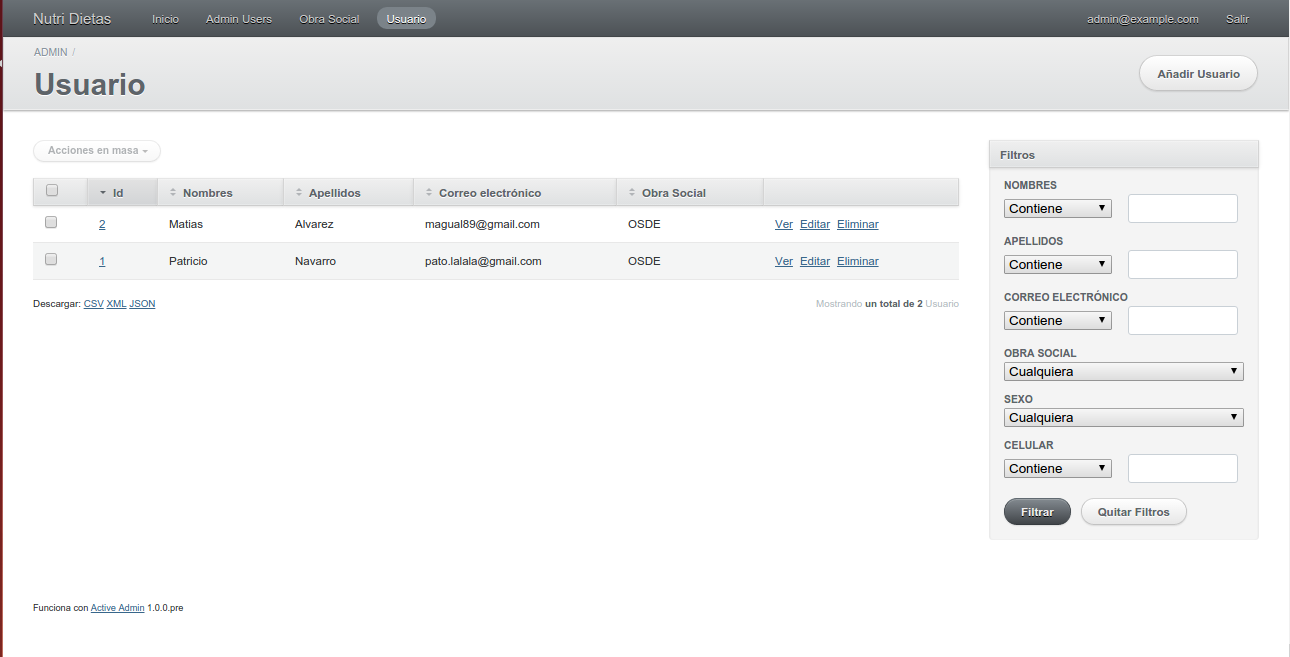
\includegraphics[scale=0.3]{paciente.png}
\end{center}

\subsection{Obra Social (Administrador)}
\begin{center}
	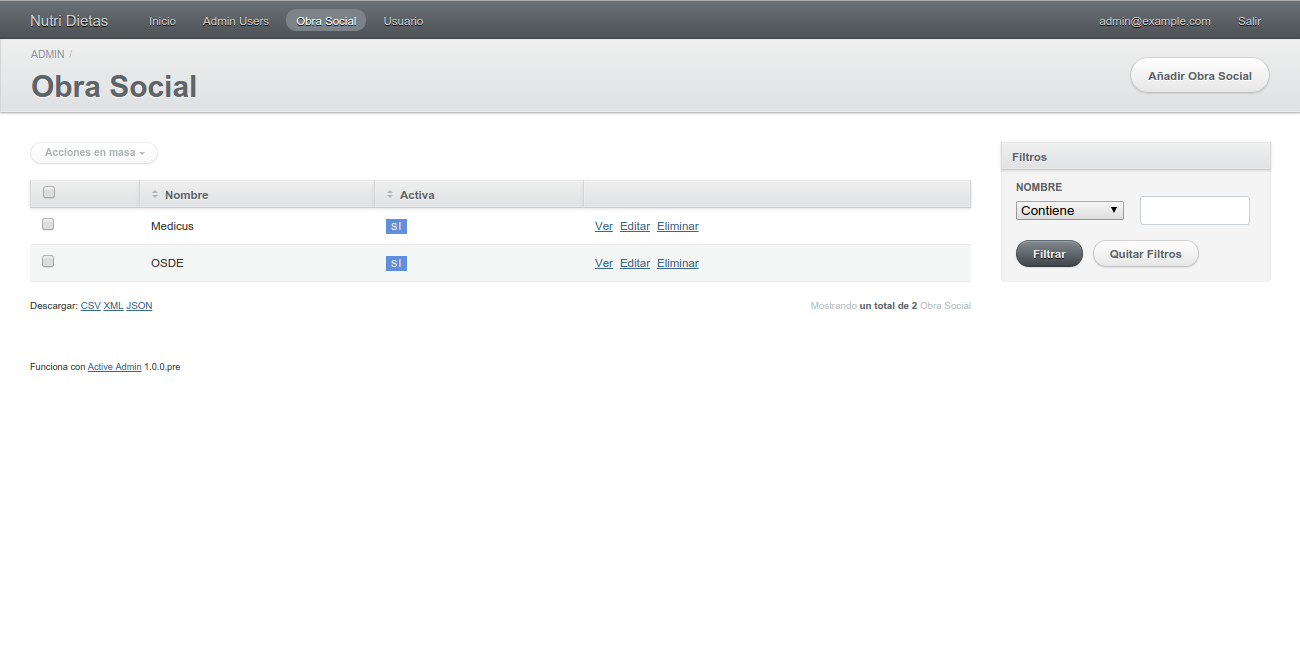
\includegraphics[scale=0.3]{obra_social.png}
\end{center}

\subsection{Peso minimo/ Peso maximo (Administrador)}
\begin{center}
	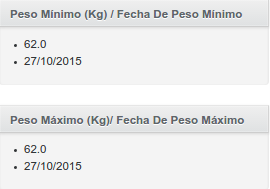
\includegraphics[scale=0.3]{minimo_maximo.png}
\end{center}

\subsection{Planes  (Administrador)}
\begin{center}
	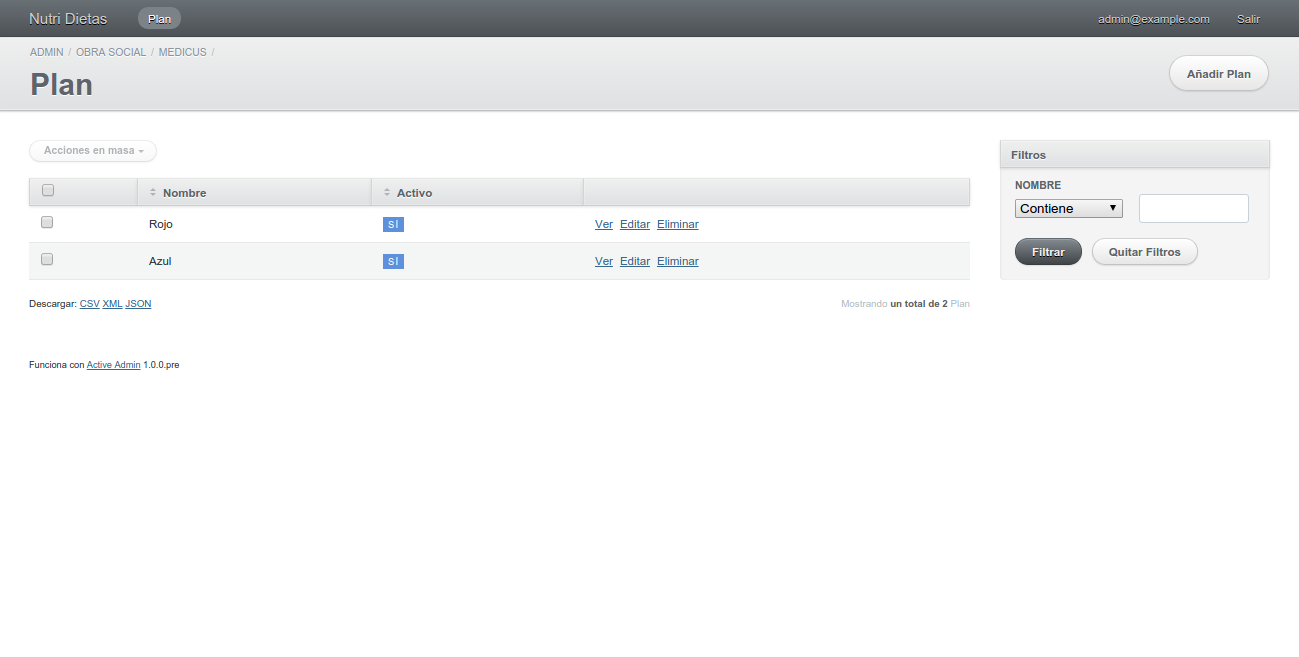
\includegraphics[scale=0.3]{planes.png}
\end{center}
 
\subsection{Historial (Administrador)}
\begin{center}
	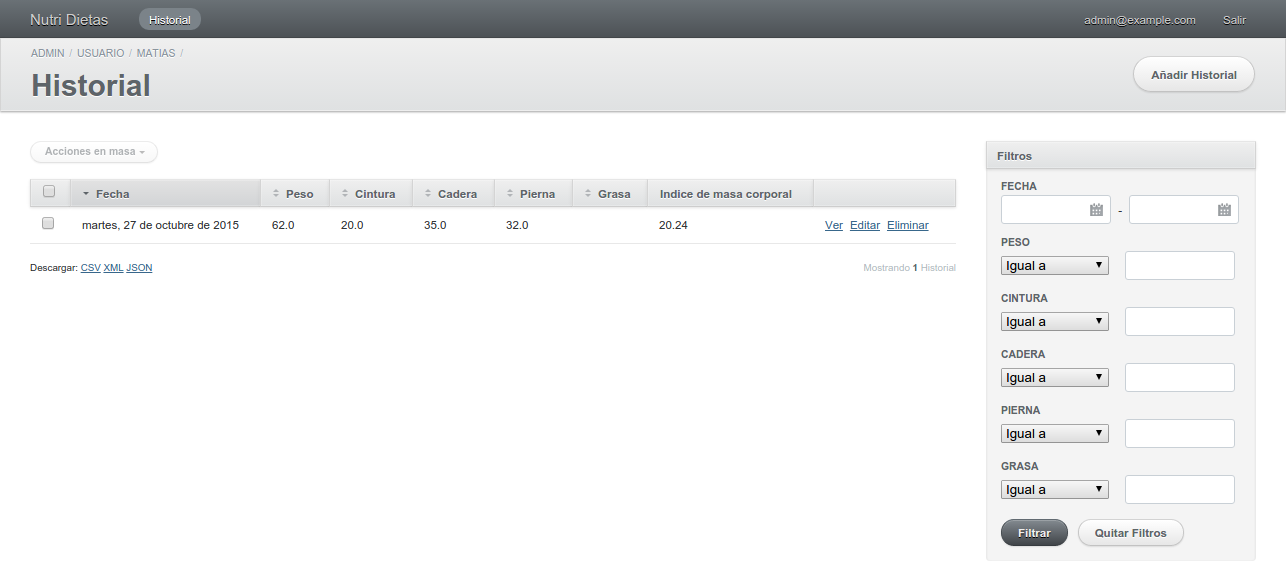
\includegraphics[scale=0.3]{historial.png}
\end{center}



\section{Metodología}
Para el desarrollo del proyecto se utilizo la metodología Scrum, en la cual se va desarrollando el producto de manera incremental y se puede ir evaluando sus resultados.\\
Esta metodología permite trabajar a los desarrolladores en conjunto con los clientes, esto permite ir notificando al grupo de trabajo sobre nuevas tareas a realizar o incluso cambios que se necesiten o mejores de algo ya realizado. Se realiza una lista de prioridades las cuales se deben trabajar sobre estas de acuerdo a su orden establecido.\\
Cada etapa del desarrollo fue planificada y se le presento al cliente para que pueda brindarnos su feedback.\\
Al finalizar cada sprint se le entrego al tutor un informe de avance especificando las tareas realizadas, features completas, estado de los bugs que posea la aplicación, gestión de riesgos y alcance del próximo sprint.

\section{Inconvenientes}
En el transcurso del proyecto se presentaron diversos inconvenientes en la realización del mismo, algunos producto de nuestra inexperiencia desarrollando aplicaciones a medida del cliente y otros propios de este tipo de proyectos.

\subsection{Captura de requisitos}
La ingeniería de requisitos es un proceso especializado que se realiza en un dominio para documentar las características que debe cumplir un producto software y transformarlas en una especificación. El documento de especificación de requisitos debe cubrir la representación y comprensión del ambiente específico y debe contener todas las funciones esenciales (funcionalidad delimitada) del software de manera rastreable, no ambigua, con independencia de los requisitos no funcionales y de las restricciones de diseño.\cite{lopez}

Durante el proceso de desarrollo se le dedico gran parte del trabajo inicial a interpretar y canalizar las necesidades del cliente. Presentándose un problema frecuente en el desarrollo de software, cuando el cliente no sabe concretamente que es lo que necesita y depende de los desarrolladores orientar esa necesidad a un producto útil y de calidad. 

\subsection{Entendimiento del modelo de negocio}
Para generar soluciones de calidad y dejar un cliente satisfecho es fundamental que el desarrollador posea un cierto conocimiento del modelo del negocio del cliente, sin convertirse este en un experto. En este caso nos encontramos con un mundo desconocido para nosotros, como lo es el de la nutrición. Donde tuvimos que entender algunos conceptos angulares, sobre su especialidad, de forma tal de poder comunicarnos con el cliente de forma clara.

\subsection{Integración sistema de turnos}
Al trabajar en una estructura híbrida donde se conservo parte del diseño antiguo, fue necesario el desarrollo de módulos que interconectaran estas distintas tegnologias. En nuestro caso se trato de conectar una base de datos de usuarios PostgreSQL administrada desde el framework (Ruby on Rails) con una base MySQL donde se encontraba la administración de los turnos. 

Al tratarse de distintas tegnologias, incompatibles entre si, donde ambos deben encontrarse sincronizados y para no volver a diseñar el sistema de turnos desde cero, se opto por sincronizar las bases de forma remota. Es decir, nuestra aplicación generara gestionara la base de turnos (Alta, Baja, Modificación) corriendo un servicio de Ruby, cada vez que se realice un cambio en la base de nuestra aplicación que debiera impactar en el sistema de turnos. 

\subsection{Presentación}
Desarrollar un producto comercial, donde la vista y presentación ante el usuario final es de suma importancia, requiere una gran atención en el detalle. En nuestro caso, al tratarse de una aplicación web esto se dio mediante la correcta selección de temas, imágenes y mas difícil aun, el desarrollo en CSS (Cascading Style Sheets). 
La puesta a punto de estos detalles visuales insume una gran cantidad de tiempo y esfuerzo al desarrollador que no se encuentra desarrollando este tipo de aplicaciones de forma habitual y continua. Buscando un balance entre esfuerzo y tiempo requeridos con la visual deseada.

\section{Conclusiones}
Durante el proceso de realización de este trabajo se pudo adquirir conocimiento y experiencia en ciertos temas, tal vez, poco de desarrollados durante la carrera. Pero que serán de gran utilidad para nuestro desarrollo como profesionales de Ingenieria Informatica. Se destacan fundamentalmente los aspectos relacionados con la "`Metodologia"' y el "`Analisis de Tiempos"'

\subsection{Metodología}


\subsection{Análisis de Tiempos}
Los problemas planteados en la sección precedente, así como la dificultad para concertar reuniones (fundamentales por la metodología utilizada)hicieron que se produjera un gran desfase entre los tiempos estimados de desarrollo y los tiempos finales. Estos inconvenientes tal vez podrían solventarse de mejor manera si se planteara la duración del proyecto en función de los sprints realizados en vez de plantearlo en días. De esta forma, el tiempo total del proyecto quedaría supeditado a la disponibilidad del cliente de concertar reuniones con los desarrolladores.
Otro inconveniente en la estimación del tiempo fue la elección de herramientas de desarrollo en las cuales no desarrollamos habitualmente, a pesar de que esto se tuvo en cuenta al momento de hacer la estimación de la duración del proyecto esta no fue eficaz. Esto, tal vez, podría mejorarse si las herramientas y tegnologias elegidas fueran ampliamente conocidas por los desarrolladores.

\appendix
\appendixpage
\section{Minuta de Reunion I}

\textbf{Fecha: }01/12/2014\\

	En la reunion se escucho las necesidades del cliente, sobre el sistema que estaba necesitando, y se avanzo en el entendimiento del negocio. Tambien fue de vital importancia comprender el estado de la cuestion actual, en referencia a las herramientas informaticas utilizadas en la actualidad para suplir el trabajo deseado de nuestro sistema. Se observo que este ultimo era de una tegnologia un poco anticuada y rudimentaria. Tambien pudo verse que el cliente poseia un alto grado de automatizacion en sus procesos, y lo requerido de nuestro sistema era la integracion y refactorizacion de todas estas piezas automatizadas.

Luego de la charla se comentó los temas a desarrollar en el próximo Sprint:
\begin{enumerate}
	\item Desarrollo de mockups y planteo de la solucion.
	\item Seleccion, instalacion y puesta a punto de la infrastructura necesaria. 
\end{enumerate}

\section{Minuta de Reunion II}

\textbf{Fecha: }27/12/2014\\

\begin{enumerate}
\item En la reunion se presento la propuesta formal al cliente, junto con las capturas de pantalla del prototipo. El cual fue aceptado por el cliente.
\item Se introdujo al cliente en la tegnologia a ser utilizada.
\end{enumerate}

\begin{flushleft}
Luego de la charla se comentó los temas a desarrollar en el próximo Sprint:
\end{flushleft}

\begin{enumerate}
	\item Desarrollar todo el ambiente de trabajo.
	\item Desarrollar la administración de pacientes. 
\end{enumerate}

\section{Minuta de Reunion III}

\textbf{Fecha: }20/01/2015\\

En la reunión se mostraron los avances sobre los objetivos del Sprint 2:
\begin{enumerate}
\item Desarrollar todo el ambiente de trabajo como el entorno, estructura de archivos, mapeo entre entidades, entendimiento de negocio. Se explicó al cliente directamente con la computadora como sería la manera de operar el sistema (vía Web). Esto fue aceptado satisfactoriamente por el cliente. Se le respondió algunas dudas que tenía. 
\item Desarrollar la administración de pacientes. Esto abarca el alta, baja y modificación de los mismos como así también la ubicación en el sistema y pantallas necesarias para lograr esto. Se pidió detalles sobre la información que necesitan cargar para el manejo de datos. Se tomó nota de ciertas especificaciones que querían para esta administración. Se nos definió como de fundamental importancia en este punto ciertos aspectos del funcionamiento del negocio que debíamos implementar correctamente. 
\end{enumerate}

\begin{flushleft}
Luego de la charla se comentó los temas a desarrollar en el próximo Sprint:
\end{flushleft}

\begin{enumerate}
	\item Corregir situaciones planteadas por el Cliente. 
	\item Implementar el manejo de usuarios de acuerdo al modelo de negocio.
	\item Desarrollar el manejo de dietas. 
\end{enumerate}

\section{Minuta de Reunion IV}

\textbf{Fecha: }03/04/2015\\

En la reunión se mostraron los avances sobre los objetivos del Sprint 3:
\begin{enumerate}
\item Desarrollo del sistema de registracion de usuarios, cumpliendo con todos los requisitos del modelo de negocio.  
\item Desarrollar la administración de dietas. Esto abarca la asginacion, visualisacion y descarga de dietas por parte de los pacientes. Las dietas son asginadas por la licenciada una vez que el paciente ha asistido al consultorio y nunca previamente. Pudiendo ella desde una interfaz de admin agregar o quitar dietas a su disposicion. En esta parte tambien se asigna y modifican las cantidades correspondientes a cada dieta.
\item Aspectos de visualisacion los cuales fueron mejorados en este sprint.
\end{enumerate}

\begin{flushleft}
Luego de la charla se comentó los temas a desarrollar en el próximo Sprint:
\end{flushleft}

\begin{enumerate}
	\item Corregir situaciones planteadas por el Cliente. 
	\item Mejora de la visualisacion de las dietas.
	\item Implementacion de registro de medidas de los pacientes. 
\end{enumerate}

\section{Minuta de Reunion V}

\textbf{Fecha: }20/05/2015\\

En la reunión se mostraron los avances sobre los objetivos del Sprint 4:
\begin{enumerate}
\item Se mejoro el panel del administrador para cumplir con los requisitos impuestos por el cliente.
\item Se refactoriso la visualizacion de las dietas para servir mejor a los requisitos del cliente.
\item Se comenzo el desarrollo del manejo de los datos historicos de los pacientes. Se creo un modelo para contener esta informacion y se bosquejo una pagina donde los usuarios realizaran las cargas.
\end{enumerate}

\begin{flushleft}
Luego de la charla se comentó los temas a desarrollar en el próximo Sprint:
\end{flushleft}

\begin{enumerate}
	\item Corregir situaciones planteadas por el Cliente. 
	\item Mejora de la visualisacion de  carga de medidas.
	\item Implementacion completa del registro de medidas de los pacientes. 
\end{enumerate}

\section{Minuta de Reunion VI}

\textbf{Fecha: }04/09/2015\\

En la reunión se mostraron los avances sobre los objetivos del Sprint 5:
\begin{enumerate}
\item Se implemento en el panel del administrador la posibilidad de visualizar de las medidas cargadas por los usuarios.
\item Se mejoro la pantalla de carga de medidas por parte de los usuarios.
\item Se realizaron mutiples fixes y mejoras en las funcionalidades como en la visualizacion del sitio.
\end{enumerate}

\begin{flushleft}
Luego de la charla se comentó los temas a desarrollar en el próximo Sprint:
\end{flushleft}

\begin{enumerate}
	\item Corregir situaciones planteadas por el Cliente. 
	\item Cambio importante en las cargas de las medidas para cumplir correcta e eficientemente con el modelo de negocio.
	\item Realizacion de los graficos en funcion de los datos historicos cargados.
	\item Agregar fecha de peso minimo y maximo historico.
	\item Dividir las dietas en varios tipos distintos algunas excluyentes entre si.
\end{enumerate}

\section{Minuta de Reunion VII}

\textbf{Fecha: }25/09/2015\\

En la reunión se mostraron los avances sobre los objetivos del Sprint 6:
\begin{enumerate}
\item Corregir situaciones planteadas por el Cliente.
\item Cambio importante en las cargas de las medidas para cumplir correcta e eficientemente con el modelo de negocio.
\item Realización gráficos estadísticos en función de los datos históricos cargados.
\item Agregar peso mínimo y máximo histórico, y fecha de los mismos
\item Clasificar las distintas dietas en subconjuntos, para facilitar su administración
\item Se cargaron en la página todos los archivos PDF’s correspondientes a cada una de las dietas.
\item Se realizaron mejoras a nivel “look and feel” de la plataforma.
\item Se removió el ingreso del porcentaje de masa corporal desde la vista de usuario.
\end{enumerate}

\begin{flushleft}
Luego de la charla se comentó los temas a desarrollar en el próximo Sprint:
\end{flushleft}

\begin{enumerate}
	\item Agregar filtro para usuarios por Obra Social en la vista de administrador. 
	\item Agregar filtro para usuarios por Plan en la vista de administrador.
	\item Rediseño del formulario de edición de usuario.
	\item Rediseño del formulario de alta de usuario para selección de Obra Social y Plan correspondiente a la misma
\end{enumerate}

\section{Minuta de Reunion VIII}

\textbf{Fecha: }12/10/2015\\

En la reunión se mostraron los avances sobre los objetivos del Sprint 7:
\begin{enumerate}
\item Agregar filtro para usuarios por Obra Social en la vista de administrador.
\item Agregar filtro para usuarios por Plan en la vista de administrador.
\item Rediseño del formulario de edición de usuario.
\item Rediseño del formulario de alta de usuario para selección de Obra Social y Plan correspondiente a la misma.
\item Resolución de bugs en formularios de administrador y de registración de usuario.
\end{enumerate}

\begin{flushleft}
Luego de la charla se comentó los temas a desarrollar en el próximo Sprint:
\end{flushleft}

\begin{enumerate}
	\item Agregar ABM de Obras Sociales a la vista de administrador
	\item Agregar ABM de Planes a la vista de administrador.
	\item Agregar control de estado sobre las Obras Sociales (activas/inactivas).
	\item Agregar control de estado sobre los Planes (activo/inactivo).
	\item Quitar la funcionalidad para que un usuario pueda editar su email.
	\item Pruebas de stress sobre la plataforma, generación de carga de datos históricos.
\end{enumerate}

\section{Minuta de Reunion IX}

\textbf{Fecha: }27/10/2015\\

En la reunión se mostraron los avances sobre los objetivos del Sprint 8:
\begin{enumerate}
\item Agregar ABM de Obras Sociales a la vista de administrador.
\item Agregar ABM de Planes a la vista de administrador.
\item Agregar control de estado sobre las Obras Sociales (activas/inactivas).
\item Agregar control de estado sobre los Planes (activo/inactivo).
\item Quitar la funcionalidad para que un usuario pueda editar su email.
\item Pruebas de stress sobre la plataforma, generación de carga de datos históricos.
\end{enumerate}

\begin{flushleft}
Luego de la charla se comentó los temas a desarrollar en el próximo Sprint:
\end{flushleft}

\begin{enumerate}
	\item Verificar funcionamiento de la aplicación sobre dispositivos móviles.
	\item Agregar nueva categoría para el índice de masa corporal.
	\item Permitir que desde la vista de administrador se puedan agregar comentarios sobre la consulta realizada al paciente.
	\item Agregado de nuevas dietas al sistema.
	\item Agregado de tooltips sobre las imágenes que representan a las diferentes dietas en la vista del usuario final.	
	\item Realizar integración con sistema de turnos existentes para poder obtener la fecha del próximo turno.
\end{enumerate}

\section{Minuta de Reunion X}

\textbf{Fecha: }18/11/2015\\

En la reunión se mostraron los avances sobre los objetivos del Sprint 9:
\begin{enumerate}
\item Verificar funcionamiento de la aplicación sobre dispositivos móviles.
\item Agregar nueva categoría para el índice de masa corporal.
\item Permitir que desde la vista de administrador se puedan agregar comentarios sobre la consulta realizada al paciente.
\item Agregado de nuevas dietas al sistema.
\item Agregado de tooltips sobre las imágenes que representan a las diferentes dietas en la vista del usuario final.
\item Realizar integración con sistema de turnos existentes para poder obtener la fecha del próximo turno.
\end{enumerate}

\begin{flushleft}
Luego de la charla se comentó los temas a desarrollar en el próximo Sprint:
\end{flushleft}

\begin{enumerate}
	\item Realizar scripts para obtener la información de archivos xls actuales y la información de la base de datos actual.
	\item Migrar los datos obtenidos a la base de datos de la plataforma.
	\item Agregar confirmación del alta de usuario vía email.
	\item Corregir error en la eliminación de Obra Social desde el administrado
\end{enumerate}

\section{Minuta de Reunion XI}

\textbf{Fecha: }03/12/2015\\

En la reunión se mostraron los avances sobre los objetivos del Sprint 10:
\begin{enumerate}
\item Realizar scripts para obtener la información de archivos xls actuales y la información de la base de datos actual.	
\item Migrar los datos obtenidos a la base de datos de la plataforma.
\item Agregar confirmación del alta de usuario vía email.
\item Corregir error en la eliminación de Obra Social desde el administrador
\end{enumerate}

\begin{flushleft}
Luego de la charla se comentó los temas a desarrollar en el próximo Sprint:
\end{flushleft}

\begin{enumerate}
	\item Pruebas de aceptación sobre la plataforma.
	\item Alta de dominio web.
	\item Puesta en producción de la plataforma.
\end{enumerate}


\begin{thebibliography}{4}

\bibitem{carrera} Plan de Carrera de Ingeniería Informática, Universidad de Buenos Aires (UBA), Argentina. \url{http://www.fi.uba.ar}
\bibitem{computacion} Departamento de Computación, Av. Paseo Colón 850 - 4to. piso - C1063ACV - Buenos Aires - Argentina
\bibitem{estrada}
Hugo Estrada, Alicia Martínez, Oscar Pastor, Juan Sánchez
\emph{Generación de Especificaciones de Requisitos de Software a partir de Modelos de Negocios: un enfoque basado en metas},
 Universidad Politécnica de Valencia,España.
\bibitem{lopez}
Oscar López,Miguel Ángel Laguna, José Manuel Marqués
\emph{Generación Automática de Casos de Uso para Desarrollo de Software Basado en Reutilización}
Instituto Tecnológico de Costa Rica, Costa Rica.

\end{thebibliography}

\end{document}
